\graphicspath{{./images/chap2/}}
% Related Literature and Studies
% * Organized to cover specific problem
% * how it helps the current study/how it relates
\chapter{Related Work} % (fold)
\label{cha:related_work}

\section{Sloop}

\subsection{Information Retrieval System}

The field of information retrieval emerges from the attempt to provide
information access. From the academic perspective, information retrieval (IR)
is a principled approach of finding desired materials of an \emph{unstructured}
nature from within large collections. The fact that it allows more flexible
query operations makes IR a dominant form of information access in practice,
compare to database-style searching. Additionally, IR supports ranked
retrieval, where it outputs the best answers given a query.

The preceding properties make information retrieval an obvious solution for
animal identification task. Tracking population and dispersal of a species from
images requires manually identifying all the individuals animals in the images.
Traditionally, this involves an arduous work of comparing thousands of images.
However, with Sloop, a pattern retrieval engine that can preprocess the images
and output an initial possible ranking, the time required to spend on going
through all the image pairs one by one could be reduced by an order of
magnitude.

\subsection{Sloop Architecture} Sloop is a distributed image retrieval system.
The system is divided into two major components:

\begin{figure}[ht]
  \centering
  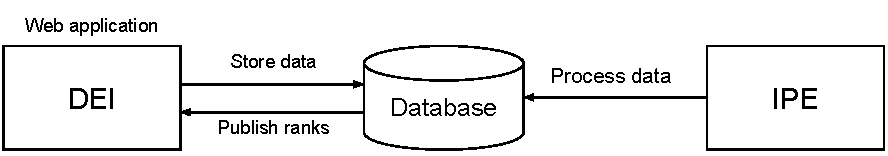
\includegraphics[width=\textwidth]{sloop/system}
  \caption{Score Distribution}
  \label{fig:sloop_overview}
\end{figure}

\begin{enumerate}
	\item Data Exchange and Interaction (DEI)
    DEI is a web application that provides the user interface that allows
    biologists to upload data onto sloop databases.
	\item Image Processing Engine (IPE)
    IPE processes the data stored in the databases and generate descriptors
    that represent identities of the images.
\end{enumerate}


Sloop identifies each animal on individual base. This provides the similarity
ranking of the images, within the same species, in the database relative to the
animal in a given image A. Effectiveness of such identification system heavily
depends on the choice of features on which the machine learning algorithms are
applied.

Current Sloop uses Scale Invariant Feature Transform (SIFT)~\cite{lowe04} to
perform such images ranking. Given an image and the four fiducial key points
annotated by the biologists, Sloop transforms the images into SIFT object and
compare it among the SIFTs of the existing images stored in the database, using
Euclidean distance. After the ranking is generated, the biologists then look at
the top matches and confirm whether the given pairs of images are matches or
non-matches.

While SIFT is still interesting for tasks that speed and simplicity are of
major concerns, it requires tremendous amount of manual effort and training.
Recent studies and competition results have proved that features learned via
convolutional neural networks (CNN) outperform previous descriptors, including
SIFT, on classification tasks by a wide margin~\cite{fisher14}. Therefore,
replacing SIFT with convolutional neural networks seem to be a viable
improvement to the system.

\section{Relevance Feedback}

Relevance Feedback is a technique that involves users in the retrieval process.
Specifically, given a query that returns a set of initial results, the system
takes user feedback on the initial results to improve the results returned from
the later iterations when given the same or related
query~\cite{manning2008introduction}.

\subsection{Crowdsourcing}

Crowdsourcing market is a platform takes advantage of collective intelligence
of the online community. Crowdsourcing has gained popularity as an inexpensive
and efficient method to accomplish certain tasks that are usually difficult for
machines alone to complete.

In a crowdsourcing market, there are three parties involved:
\begin{enumerate}
	\item Workers
	\item Requesters
	\item Crowdsourcing platform
\end{enumerate}

\emph{Requesters} submit tasks with the amount of \emph{reward} that they are
willing to pay \emph{workers} upon the completion of the tasks. Some workers
maybe better than others at certain tasks. In other words, some tasks maybe
more difficult than others for some workers. The platform provides the
environment for the worker and requesters to interact. All parties gain more
information about one another and the tasks, and make repeated decision
overtime.

\section{Image Recognition}

\subsection{Convolutional Neural Network}

Convolutional Neural Network is a special kind of multi-layer neural networks,
whose task is specialized to capture and encode visual patterns directly from
raw pixel images~\cite{lecun95}.

\subsection{Face Verification and Siamese Network}

The problem of finding matching image pairs from the database given an input
image, can be reduced to following \emph{decision problem}:
\begin{quote}
\centering
Given two images A and B, is the animal in image A the same individual as the
animal in image B?
\end{quote}

Our problem is somewhat similar to the face verification problem, which
involves accepting or rejecting an identity claim based on the image of a human
face. There are two major differences between animal identification and face
verification. First, the animal pattern has finer-grained details and some can
be very subtle that they fuse into the background. Second, the pattern of each
individual does not share same overall structure as human face does. This is
similar to identifying an identical twin by their blemishes except for, in this
case, we have very high-order of multiple births.

Most current face verification methods use hand-crafted features, which are
often combined to improve the validation performance. In~\cite{chopra05},
Chopra presented a new framework, \emph{Siamese Network}, as a solution to this
problem. He proposed a training method that is used to learn a similarity
metric from the data with the contrastive loss function, comprised of the sum
of the \emph{magnitude of the difference between the features vectors} of the
incorrect guesses. This loss function encourages matching pairs to be close
together in feature space while pushing non-matching pairs apart. However, it
may not be the best option in our case because the difference in each feature
contributes equal weight to the loss, whereas in our model, each feature may
require different weights in the loss function that is not proportional to the
weight learned in the convolutional network.

% chapter related_work (end)
